\documentclass{beamer}

\mode<presentation>
{\usetheme{boxes}}

\usepackage{array}
\usepackage{times}
\usepackage{graphicx}
\usepackage{hyperref}
\usepackage{listings}
\usepackage{relsize}
\usepackage{ragged2e}
\usepackage[T1]{fontenc}

\lstdefinestyle{customc}{
  belowcaptionskip=1\baselineskip,
  breaklines=true,
  frame=L,
  xleftmargin=\parindent,
  language=C,
  showstringspaces=false,
  basicstyle=\footnotesize\ttfamily,
  keywordstyle=\bfseries\color{green!40!black},
  commentstyle=\itshape\color{purple!40!black},
  identifierstyle=\color{blue},
  stringstyle=\color{red},
}
\lstdefinestyle{custombash}{
  belowcaptionskip=1\baselineskip,
  breaklines=true,
  frame=L,
  xleftmargin=\parindent,
  language=bash,
  basicstyle=\footnotesize\ttfamily,
  showstringspaces=false,
  commentstyle=\itshape\color{purple!40!black},
  keywordstyle=\itshape\color{green!40!black},
  identifierstyle=\color{blue},
  stringstyle=\color{orange},
}

\usebackgroundtemplate
{
  \hbox to \paperwidth{\hfil
\includegraphics[width=4in,
      height=\paperheight]{wildcat_transparent.jpg}\hfil}
}

\title{PHYS 105 Lecture 6: Variable Operators, While Loops, 
  Numerical Integration}
\author{Tom McClintock \\
	Dept. of Physics\\
	University of Arizona
}
\date{\today}

\begin{document}

\begin{frame}
  \titlepage
\end{frame}

\begin{frame}
  \frametitle{Last time}
  \begin{itemize}
    \item Character strings
    \item Arrays
  \end{itemize}
\end{frame}

\begin{frame}
  \frametitle{This time}
  \begin{itemize}
    \item Variable operations
    \item While loops
    \item Numerical integration
  \end{itemize}
\end{frame}

\begin{frame}[fragile]
  \frametitle{Variable Operations}
  A few weeks ago we learned the basic mathematical operations.\\
  There are more operations that can be performed on variables in
  C. The reason for this is primarily to allow for shorthand expressions.\\
  That is, you can write a mathematical operation more quickly.\\
  For instance:
  \begin{lstlisting}[style=customc]
    x = x + 3; //Add 3 to x.
    x += 3;    //This means the same thing
  \end{lstlisting}
\end{frame}

\begin{frame}[fragile,allowframebreaks]
  \frametitle{variableops.c}
  Here is a list of all variable operations:
  \lstinputlisting[style=customc]{variableops.c}
\end{frame}

\begin{frame}[fragile]
  \frametitle{While loops}
  Two weeks ago we learned how to use for loops. Very rarely, there
  are moments when the \textbf{stopping condition} isn't dictated by
  a counter. \\
  In these cases, it is more appropriate to use a \textbf{while} loop.\\
  Here is the format for such a loop:
  \begin{lstlisting}[style=customc]
    ...
    while(condition){
      ...// Inside while loop
      ...// Only happens when condition is true
    }
    ...// Outside loop
  \end{lstlisting}
\end{frame}

\begin{frame}[fragile,allowframebreaks]
  \frametitle{While loops cont.}
  Here is a previous in class assignment
  rewritten with a \textbf{while} loop.
  \lstinputlisting[style=customc]{whileloop.c}
  In general you should use for loops, since you have more
  explicit control over when it stops and how it iterates.
\end{frame}

\begin{frame}
  \frametitle{Numerical Integration}
  Of great importance in physics is our ability to perform integrals.\\
  So far in your education you have been given instructions on how
  to perform integrals analytically.\\
  \vspace{12pt}
  In for real big people research, integrals become \textit{impossible}
  to do analytically. By that I don't mean the kind of impossible 
  that can be solved by a genius, I mean literally impossible.\\
  \vspace{12pt}
  For this reason, \textbf{numerical integration} might be the 
  most useful tool you learn in this class.\\
  \vspace{12pt}
  No pressure!
\end{frame}

\begin{frame}
  \frametitle{Rectangle Method}
  Thankfully basic \textbf{numerical integration} is easy!\\
  The method you will use in this class is the rectangle rule.
  Essentially, the area under a curve is broken into small rectangles,
  which individually are easy to find the area of.
  The area under the curve is approximately the sum of the area of
  all of the rectangles.
  \begin{center}
    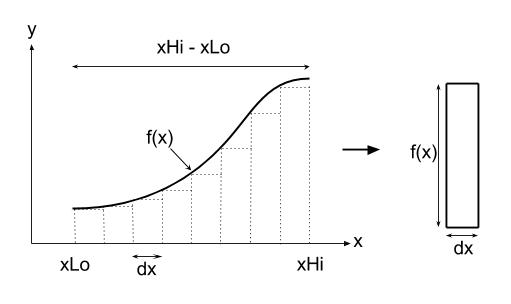
\includegraphics[width=0.5\textwidth]{rectanglemethod.jpg}
  \end{center}
\end{frame}

\begin{frame}[fragile,allowframebreaks]
  \frametitle{rectangle\_method.c}
  Here is an implementation of the rectangle method.
  \lstinputlisting[style=customc]{rectangle_method.c}
\end{frame}

\begin{frame}
  \frametitle{In class assignment}
  Integrate the function $\sin(x)$ from $0$ to $\pi$ and also from
  $0$ to $2\pi$. \\
  Note: $\pi$ can be found in the math library as well if you type
  ``M\_PI''. Also, remember to link the math library with ``-lm''!
\end{frame}

\begin{frame}
  \frametitle{Next time}
  \begin{itemize}
    \item Functions
    \item Pointers
  \end{itemize}
\end{frame}

\begin{frame}
  \frametitle{HW 4 - Trapezoid method due in 2 weeks}
  The rectangle is the most basic and most inaccurate way to do
  numerical integration. The next best way is called the Trapezoid method.
  In this method, instead of finding areas of rectangles under a curve you find
  areas of trapezoids. In terms of function evaluations and the step
  size, $dx$, this has the form:
  \begin{equation*}
    A_{trap} = \frac{dx}{2}(f(x)+f(x+dx)).
  \end{equation*}
  Implement the trapezoid method, and perform the following numerical integral:
  \begin{equation*}
    \int_{-10}^{10}\sqrt{\pi}e^{-x^2}dx.
  \end{equation*}
\end{frame}

\end{document}